% fig_ch30_wormhole_throat.tex
% Author: Computernonymouse
% Description: Morris-Thorne wormhole embedding diagram and shape function
% Shows throat geometry connecting two spacetime regions
% Mathematical basis: ds^2 = -e^(2Phi)c^2dt^2 + dr^2/(1-b(r)/r) + r^2 dOmega^2

\documentclass[tikz,border=10pt]{standalone}
\usepackage{pgfplots}
\usepackage{amsmath,amssymb}
\usepackage{xcolor}
\pgfplotsset{compat=1.18}
\usetikzlibrary{arrows.meta,decorations.pathreplacing,calc,patterns,backgrounds,shapes,positioning}
\usepgfplotslibrary{fillbetween}

% Define custom colors for wormhole regions
\definecolor{universeA}{RGB}{70,130,180}
\definecolor{universeB}{RGB}{180,70,130}
\definecolor{exoticmatter}{RGB}{255,200,100}
\definecolor{throat}{RGB}{200,50,50}

\begin{document}
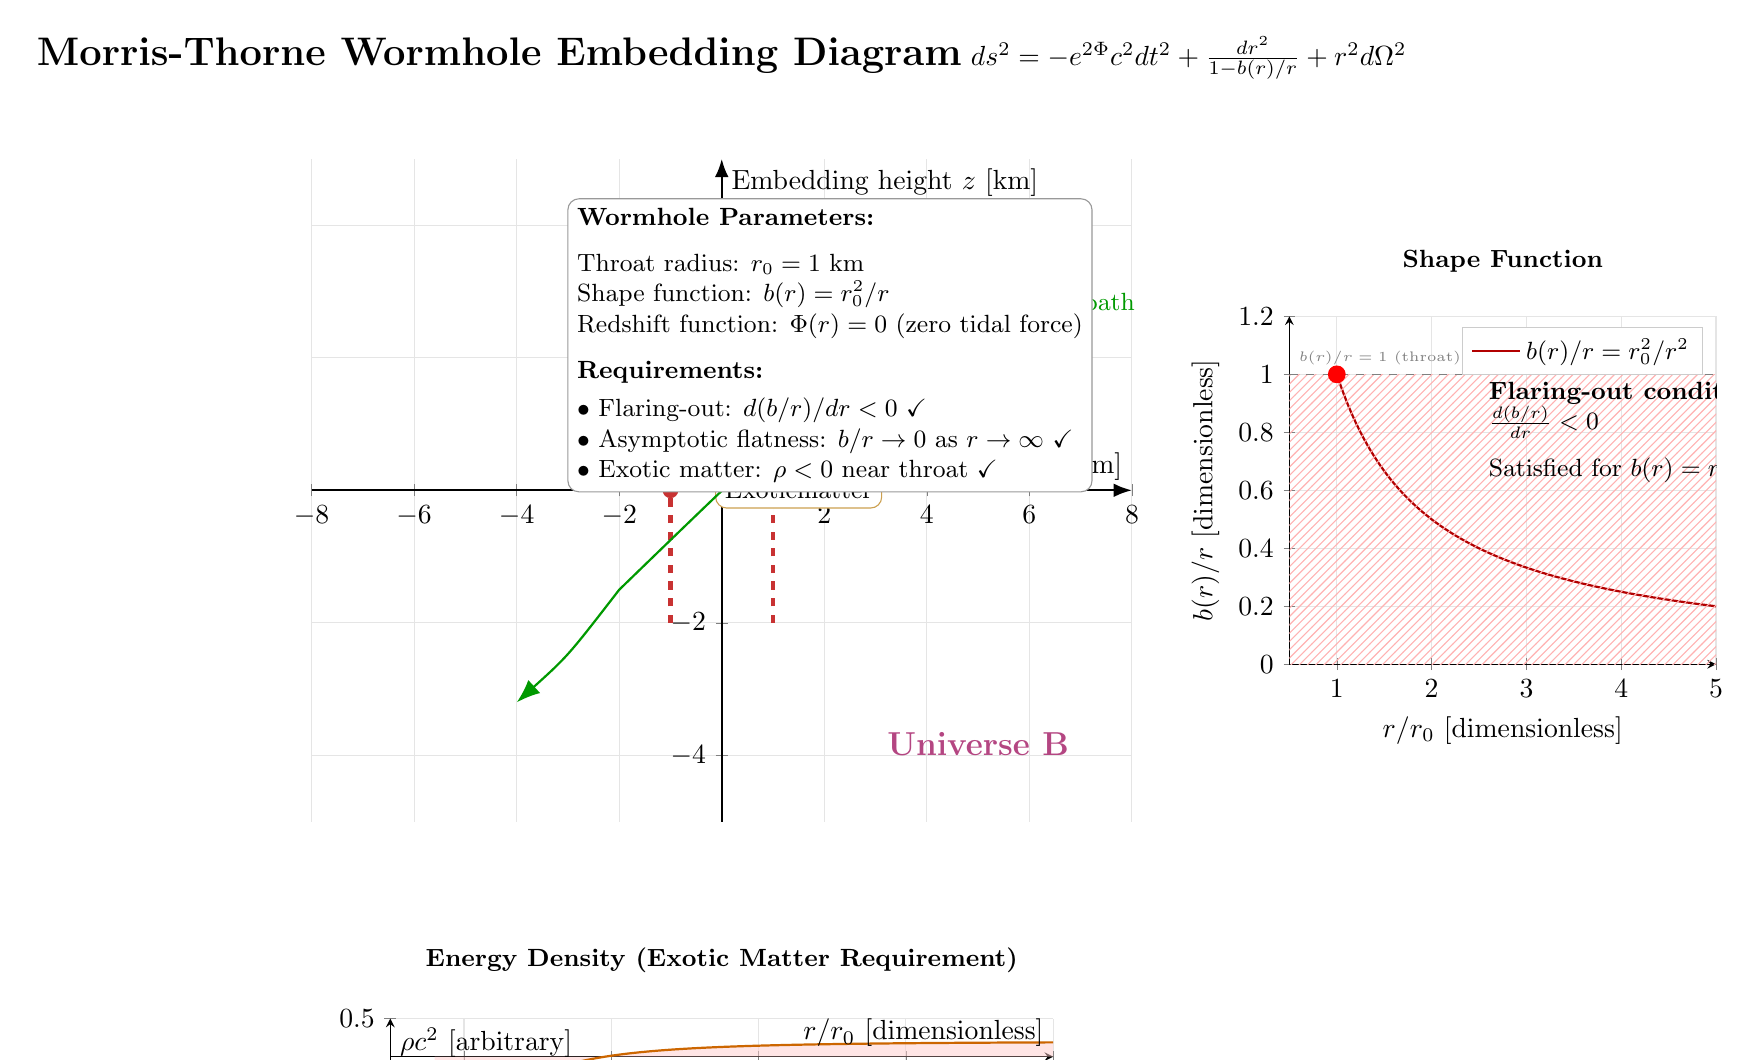
\begin{tikzpicture}

% Main embedding diagram
\begin{axis}[
    name=embedding,
    width=12cm,
    height=10cm,
    xlabel={Radial coordinate $\rho$ [km]},
    ylabel={Embedding height $z$ [km]},
    xmin=-8,xmax=8,
    ymin=-5,ymax=5,
    xtick={-8,-6,-4,-2,0,2,4,6,8},
    ytick={-4,-2,0,2,4},
    grid=major,
    grid style={gray!20},
    axis lines=center,
    axis line style={-Latex,thick},
    title={{\Large\bfseries Morris-Thorne Wormhole Embedding Diagram}\\[2mm]
           {\normalsize $ds^2 = -e^{2\Phi}c^2dt^2 + \frac{dr^2}{1-b(r)/r} + r^2d\Omega^2$}},
    title style={at={(0.5,1.08)}},
    clip=false,
    legend pos=north west,
    legend style={draw=gray!40,fill=white,fill opacity=0.9}
]

% Define shape function b(r) = r_0^2/r for simplicity
% Embedding equation: dz/dr = ± sqrt(b(r)/r / (1 - b(r)/r))
% For r_0 = 1 km (throat radius)

% Upper universe (positive z)
\addplot[
    name path=upper,
    ultra thick,
    universeA,
    domain=1:8,
    samples=100,
    smooth,
]
{sqrt((1/x - 1)) * (x > 1 ? 1 : -1) + 2};

% Lower universe (negative z)
\addplot[
    name path=lower,
    ultra thick,
    universeB,
    domain=1:8,
    samples=100,
    smooth,
]
{-sqrt((1/x - 1)) * (x > 1 ? 1 : -1) - 2};

% Mirror for negative x (left side)
\addplot[
    ultra thick,
    universeA,
    domain=-8:-1,
    samples=100,
    smooth,
]
{sqrt((1/abs(x) - 1)) * (abs(x) > 1 ? 1 : -1) + 2};

\addplot[
    ultra thick,
    universeB,
    domain=-8:-1,
    samples=100,
    smooth,
]
{-sqrt((1/abs(x) - 1)) * (abs(x) > 1 ? 1 : -1) - 2};

% Throat connection (vertical line at r = r_0)
\draw[ultra thick,throat,dashed] (axis cs:1,-2) -- (axis cs:1,2);
\draw[ultra thick,throat,dashed] (axis cs:-1,-2) -- (axis cs:-1,2);

% Shade exotic matter region
\addplot[
    name path=zero,
    draw=none,
] {0};

\addplot[
    exoticmatter,
    opacity=0.3,
] fill between[
    of=upper and lower,
    soft clip={domain=0.8:2},
];

\addplot[
    exoticmatter,
    opacity=0.3,
] fill between[
    of=upper and lower,
    soft clip={domain=-2:-0.8},
];

% Mark throat radius
\node[circle,fill=throat,inner sep=2pt] at (axis cs:1,0) {};
\node[circle,fill=throat,inner sep=2pt] at (axis cs:-1,0) {};
\node[anchor=south,font=\small\bfseries] at (axis cs:0,0.3) {Throat radius $r_0$};

% Add universe labels
\node[anchor=south,font=\large\bfseries,color=universeA] at (axis cs:5,3.5) {Universe A};
\node[anchor=north,font=\large\bfseries,color=universeB] at (axis cs:5,-3.5) {Universe B};

% Add exotic matter label
\node[draw=exoticmatter!80!black,fill=white,rounded corners,font=\small]
    at (axis cs:1.5,0) {Exotic\\matter};

% Add arrows showing traversability
\draw[-{Latex[length=3mm]},thick,green!60!black]
    (axis cs:4,2.8) .. controls (axis cs:2,1.5) and (axis cs:0,0) .. (axis cs:-2,-1.5)
    .. controls (axis cs:-3,-2.5) .. (axis cs:-4,-3.2);
\node[anchor=west,font=\small,green!60!black] at (axis cs:4.2,2.8) {Traversable path};

\end{axis}

% Shape function plot (right side)
\begin{axis}[
    at={(embedding.east)},
    anchor=west,
    xshift=2cm,
    width=7cm,
    height=6cm,
    xlabel={$r/r_0$ [dimensionless]},
    ylabel={$b(r)/r$ [dimensionless]},
    xmin=0.5,xmax=5,
    ymin=0,ymax=1.2,
    xtick={1,2,3,4,5},
    ytick={0,0.2,0.4,0.6,0.8,1,1.2},
    grid=major,
    grid style={gray!20},
    axis lines=left,
    title={\small\bfseries Shape Function},
    title style={at={(0.5,1.05)}},
    legend pos=north east,
    legend style={font=\small,draw=gray!40,fill=white}
]

% Plot b(r)/r
\addplot[
    thick,
    red!70!black,
    domain=1:5,
    samples=100,
]
{1/x};

% Mark critical point at throat
\addplot[mark=*,mark size=3pt,red] coordinates {(1,1)};

% Flaring-out condition region
\addplot[
    pattern=north east lines,
    pattern color=red!30,
    draw=none,
    domain=0.5:5,
    samples=2,
] {1} \closedcycle;

% Add condition annotations
\node[anchor=west,font=\small,align=left] at (axis cs:2.5,0.8) {
    \textbf{Flaring-out condition:}\\
    $\frac{d(b/r)}{dr} < 0$\\[2mm]
    Satisfied for $b(r) = r_0^2/r$
};

% Legend
\addlegendentry{$b(r)/r = r_0^2/r^2$}

% Horizontal line at b/r = 1
\draw[dashed,gray] (axis cs:0.5,1) -- (axis cs:5,1);
\node[anchor=south west,font=\tiny,gray] at (axis cs:0.5,1) {$b(r)/r = 1$ (throat)};

\end{axis}

% Energy density plot (bottom)
\begin{axis}[
    at={(embedding.south)},
    anchor=north,
    yshift=-2.5cm,
    width=10cm,
    height=4cm,
    xlabel={$r/r_0$ [dimensionless]},
    ylabel={$\rho c^2$ [arbitrary]},
    xmin=0.5,xmax=5,
    ymin=-2,ymax=0.5,
    xtick={1,2,3,4,5},
    ytick={-2,-1.5,-1,-0.5,0,0.5},
    grid=major,
    grid style={gray!20},
    axis lines=middle,
    title={\small\bfseries Energy Density (Exotic Matter Requirement)},
    title style={at={(0.5,1.1)}},
]

% Plot energy density (negative near throat)
\addplot[
    thick,
    orange!80!black,
    domain=0.8:5,
    samples=100,
]
{-1.5/x^3 + 0.2};

% Shade negative energy region
\addplot[
    name path=energy,
    draw=none,
    domain=0.8:5,
] {-1.5/x^3 + 0.2};

\addplot[
    name path=zero2,
    draw=none,
] {0};

\addplot[
    red!20,
    opacity=0.5,
] fill between[
    of=energy and zero2,
    soft clip={domain=0.8:5},
];

% Mark violation of null energy condition
\node[draw=red!70!black,fill=white,rounded corners,font=\small]
    at (axis cs:2.5,-0.8) {NEC violation: $\rho + p < 0$};

\end{axis}

% Add parameter box
\node[anchor=north east,draw=black!40,fill=white,rounded corners,align=left,font=\small]
    at ([xshift=-5mm,yshift=-5mm]embedding.north east) {
    \textbf{Wormhole Parameters:}\\[2mm]
    Throat radius: $r_0 = 1$ km\\
    Shape function: $b(r) = r_0^2/r$\\
    Redshift function: $\Phi(r) = 0$ (zero tidal force)\\[2mm]
    \textbf{Requirements:}\\[1mm]
    $\bullet$ Flaring-out: $d(b/r)/dr < 0$ \checkmark\\
    $\bullet$ Asymptotic flatness: $b/r \to 0$ as $r \to \infty$ \checkmark\\
    $\bullet$ Exotic matter: $\rho < 0$ near throat \checkmark
};

\end{tikzpicture}
\end{document}